\documentclass[11pt,oneside,a4paper]{article}

% Packages
\usepackage{cite}
\usepackage{graphicx}
\usepackage{subfigure}
\usepackage{float}
\usepackage{url}

\begin{document}

% paper title
% can use linebreaks \\ within to get better formatting as desired
\title{Probabilistic Robotics Lab 2 \\ Split and Merge}
%
%
% author names and IEEE memberships
% note positions of commas and nonbreaking spaces ( ~ ) LaTeX will not break
% a structure at a ~ so this keeps an author's name from being broken across
% two lines.
\author{Rodrigo~Caye~Daudt}



% make the title area
\maketitle




% Note that keywords are not normally used for peerreview papers.
%\begin{IEEEkeywords}
%IEEEtran, journal, \LaTeX, paper, template. ln505
%\end{IEEEkeywords}



%%%%%%%%%%%%%%%%%%%%%%%%%%%%%%%%%%%%%%%%%%%%%%%%%%%%%%%%%%%%%%%%%%%%%%%%%%%%%%%
\section{Introduction}
 
This report describes a basic implementation of the Split and Merge algorithm. The implementation was written in Python, and is was tested with two sets of recorded data from real robots. These datasets contained information about the robot's odometry system and laser rangefinders. The objective was to use the available data to infer characteristics of the environment in which the robot was moving.


%%%%%%%%%%%%%%%%%%%%%%%%%%%%%%%%%%%%%%%%%%%%%%%%%%%%%%%%%%%%%%%%%%%%%%%%%%%%%%%
\section{Split and Merge Algorithm}\label{doh}

The robot's laser rangefinder provides us with with a set of detected points relative to the robot at each cycle. Coupled with the odometry information we are able to calculate the coordinates of these points relative to a fixed world coordinate system (in our case, the $(x,y)$ plane). Although these points are now properly placed in our map, points are not the most appropriate data form for obstacles if we want to perform trajectory planning, SLAM, or other algorithms essential for mobile robotics. Nowadays, many algorithms exist to extract object information from the obtained cloud of points. We implemented the Split and Merge algorithm \cite{nguyen2005comparison}, which tries to split the obtained points into a set of lines, which is a data format much more appropriate for describing a map in mobile robotics.

This algorithm consists on a series of simple steps. First, the algorithm defines a line between the first and the last points in the dataset and calculates the distances between all points to this line. If the farthest point from the line exceeds a given threshold, the line will be split at that point, and the algorithm will be applied recursively to the generated subsets. Once the dataset has been split onto lines according to the defined thresholds, the function checks if the distance between sequential points in every line is smaller than another given threshold, and if so it is split even further. Finally, the lines with neighbouring points in the dataset are compared regarding distance and angle difference, and if they are similar enough they are merged.

With the right parameters, the Split and Merge algorithm transforms the dataset of points into a much smaller set of straight lone segments, which can be easily analysed for path planning, for example.

%%%%%%%%%%%%%%%%%%%%%%%%%%%%%%%%%%%%%%%%%%%%%%%%%%%%%%%%%%%%%%%%%%%%%%%%%%%%%%%
\section{Implementation}

The Python implementation of the Split and Merge algorithm followed very closely the description in Section \ref{doh}. The \textit{splitandmerge} function had as a necessary input argument the set of points that were to be split into lines. This input was done in the shape of a $2\times N$ array, where each column represented the $(x, y)$ coordinates of each detected points. The function could also be called overwriting any of the default threshold values used for the Split and Merge algorithm. The output of the function is in the shape of an $N\times 4$ array, where each line contained the $(x, y)$ coordinates of the first and last points of each line segment.


%%%%%%%%%%%%%%%%%%%%%%%%%%%%%%%%%%%%%%%%%%%%%%%%%%%%%%%%%%%%%%%%%%%%%%%%%%%%%%%
\section{Simulation Parameters and Results}

We applied the function over two different datasets, called "dataset3" and "dataset2". These datasets had different characteristics (dataset2 was much more dense, for example). Figures \ref{dataset3} and \ref{dataset2} show the result obtained using the parameters in Table 1, which were the parameters found to yield the best results for each dataset.

\begin{table}[H]
	\begin{tabular}{l | r r r r r}\label{table1}
	Dataset & split\_thres & inter\_thres & min\_points & dist\_thres & ang\_thres \\
	\hline
	dataset3 & 0.1 & 0.3 & 6 & 0.12 & 10$^{\circ}$ \\
	dataset2 & 0.01 & 0.3 & 6 & 0.12 & 10$^{\circ}$ \\
	
	\end{tabular}
	\caption{Empirically found parameters for each dataset}
\end{table}

\begin{figure}
	\centering
	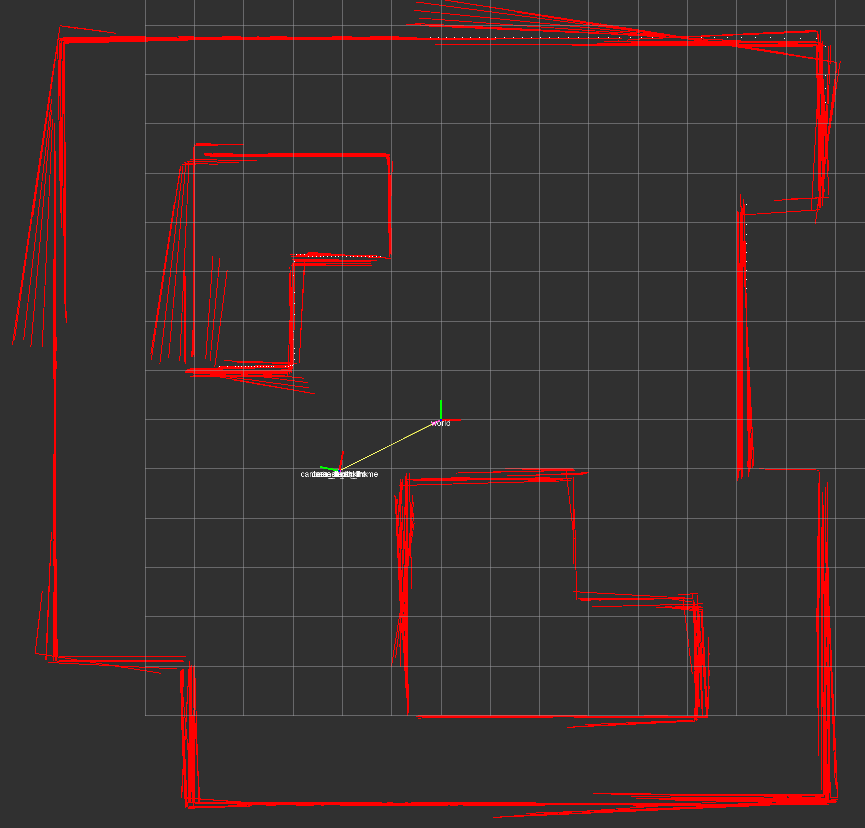
\includegraphics[width=0.8\textwidth]{figures/dataset3.png}
	\caption{Resulting lines using dataset3}
	\label{dataset3}
\end{figure}

\begin{figure}
	\centering
	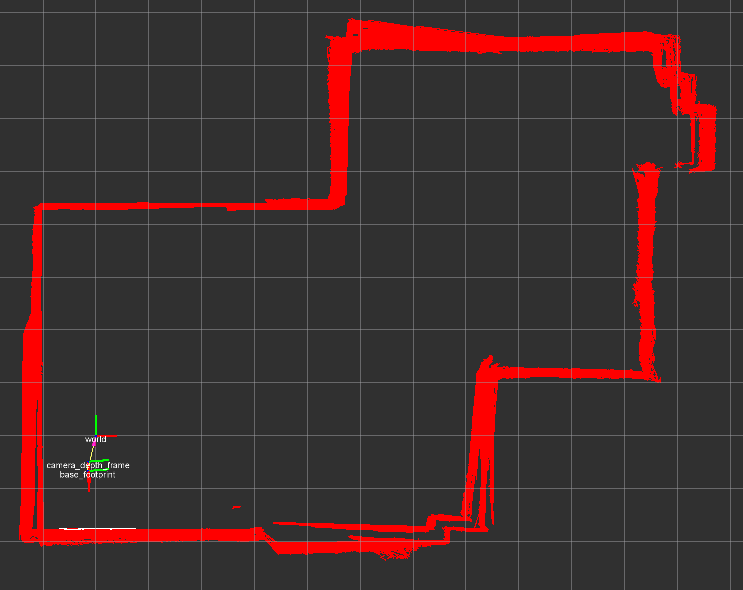
\includegraphics[width=0.8\textwidth]{figures/dataset2.png}
	\caption{Resulting lines using dataset2}
	\label{dataset2}
\end{figure}




%%%%%%%%%%%%%%%%%%%%%%%%%%%%%%%%%%%%%%%%%%%%%%%%%%%%%%%%%%%%%%%%%%%%%%%%%%%%%%%
\section{Difficulties during development}

The main difficulties encountered during the development of this work came primarily from the lack of documentation on some of the used functions. For example, the calling of the \textit{publish\_lines} function used to draw the lines had to be modified in order to keep the drawn lines on the screen, and information about how to accomplish this was hard to find. 


%%%%%%%%%%%%%%%%%%%%%%%%%%%%%%%%%%%%%%%%%%%%%%%%%%%%%%%%%%%%%%%%%%%%%%%%%%%%%%%
\section{Conclusion}

The usage of the Split and Merge algorithm was demonstrated, and we observed that it is a simple algorithm able to run in real time applications. We could also observe in the resulting images how errors in the odometry and rangefinder can result in improperly positioned points in space. Finally, we also observed that the results from this method seem to be good enough to be used for other mapping and path planning applications as long as the parameters are well tuned.



%\begin{figure}
%	\centering
%	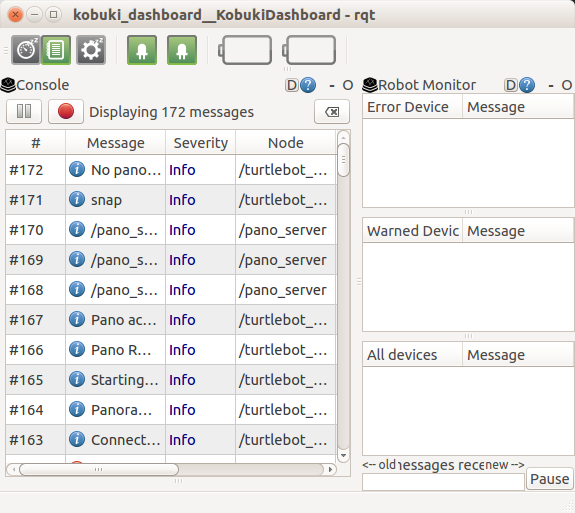
\includegraphics[width=2.5in]{figures/dashboard.png}
%	\caption{Turtlebot dashboard}
%	\label{dashboard}
%\end{figure}









%\appendices
%\section{Proof of the First Zonklar Equation}
%Appendix one text goes here.
%
%\section{}
%Appendix two text goes here.


% use section* for acknowledgement
%\section*{Acknowledgment}
%The authors would like to thank...


\bibliographystyle{IEEEtran}
\bibliography{Template_Daudt}


\end{document}


